\documentclass[12pt,a4paper]{article}

% ─── Page Layout ───────────────────────────────────────────────────────────────
\usepackage[a4paper, margin=0.8in, headheight=14pt]{geometry}

% ─── Fonts (XeLaTeX) ───────────────────────────────────────────────────────────
\usepackage{fontspec}
\usepackage{unicode-math}
\setmainfont{TeX Gyre Pagella}
\setmonofont[Scale=0.88]{TeX Gyre Cursor}
\setmathfont{Latin Modern Math}

% ─── Packages ──────────────────────────────────────────────────────────────────
\usepackage{xcolor}
\usepackage{colortbl}
\usepackage{titlesec}
\usepackage{enumitem}
\usepackage{tabularx}
\usepackage{booktabs}
\usepackage{array}
\usepackage{amsmath}
\usepackage{tikz}
\usetikzlibrary{shapes.geometric, arrows.meta, positioning, calc, fit, decorations.pathreplacing}
\usepackage{tcolorbox}
\tcbuselibrary{skins, breakable}
\usepackage{hyperref}
\usepackage{fancyhdr}
\usepackage{graphicx}
\usepackage{microtype}
\hyphenpenalty=10000
\exhyphenpenalty=10000
\sloppy
\usepackage{caption}
\usepackage{setspace}
\usepackage{multirow}
\usepackage{tocloft}

% ─── Q&A helper ────────────────────────────────────────────────────────────────
\newcommand{\Q}[1]{\textbf{#1}\par\noindent\ignorespaces}

% ─── Colour Palette ────────────────────────────────────────────────────────────
\definecolor{myred}{RGB}{196,30,58}
\definecolor{mydark}{RGB}{30,30,50}
\definecolor{mygreen}{RGB}{14,120,80}
\definecolor{myteal}{RGB}{0,130,140}
\definecolor{myamber}{RGB}{180,100,0}
\definecolor{mypurple}{RGB}{100,30,160}
\definecolor{mygray}{RGB}{246,247,249}
\definecolor{mgframe}{RGB}{180,185,200}
\definecolor{watermark}{RGB}{145,150,170}
\definecolor{hdrred}{RGB}{250,232,235}
\definecolor{hdrgreen}{RGB}{220,244,233}
\definecolor{hdrteal}{RGB}{220,242,244}
\definecolor{hdramber}{RGB}{253,242,215}
\definecolor{hdrpurple}{RGB}{238,228,255}
\definecolor{hdrgray}{RGB}{238,240,245}
\definecolor{rowalt}{RGB}{250,251,253}

% ─── Section Formatting ────────────────────────────────────────────────────────
\titleformat{\section}
  {\large\bfseries\color{myred}}{\thesection.}{0.5em}{}
  [\vspace{1pt}{\color{myred}\rule{\linewidth}{0.8pt}}]
\titleformat{\subsection}
  {\normalsize\bfseries\color{myteal}}{\thesubsection}{0.5em}{}
\titlespacing*{\section}{0pt}{18pt}{7pt}
\titlespacing*{\subsection}{0pt}{11pt}{4pt}

% ─── Paragraph ─────────────────────────────────────────────────────────────────
\setlength{\parindent}{0pt}
\setlength{\parskip}{4pt}

% ─── TOC Styling ───────────────────────────────────────────────────────────────
\renewcommand{\cfttoctitlefont}{\large\bfseries\color{myred}}
\renewcommand{\cftaftertoctitle}{\par\noindent{\color{myred}\rule{\linewidth}{0.8pt}}}
\setlength{\cftbeforetoctitleskip}{0pt}
\setlength{\cftaftertoctitleskip}{6pt}
\renewcommand{\cftsecfont}{\normalsize\bfseries\color{mydark}}
\renewcommand{\cftsecpagefont}{\normalsize\bfseries\color{mydark}}
\renewcommand{\cftsecleader}{\cftdotfill{\cftdotsep}}
\setlength{\cftbeforesecskip}{7pt}
\renewcommand{\cftsubsecfont}{\small\color{mydark}}
\renewcommand{\cftsubsecpagefont}{\small\color{mydark}}
\setlength{\cftbeforesubsecskip}{3pt}
\setlength{\cftsubsecindent}{1.4em}

% ─── Table helpers ─────────────────────────────────────────────────────────────
\renewcommand{\arraystretch}{1.45}
\setlength{\tabcolsep}{6pt}
\arrayrulecolor{mydark}
\newcolumntype{B}[1]{>{\small\bfseries\raggedright\arraybackslash}m{#1}}
\newcolumntype{Y}{>{\small\raggedright\arraybackslash}X}
\renewcommand{\tabularxcolumn}[1]{m{#1}}

% ─── Header / Footer ───────────────────────────────────────────────────────────
\pagestyle{fancy}
\fancyhf{}
\fancyhead[L]{\small\color{myred}\textbf{HS-HU601}\;\color{mydark}--- Economics for Engineers}
\fancyhead[R]{\small\color{myteal}\textbf{Module 4 Notes}}
\fancyfoot[C]{\small\color{mydark}\thepage}
\fancyfoot[R]{\small\color{watermark}\textit{\copyright\ Biraj}}
\renewcommand{\headrulewidth}{0.5pt}
\renewcommand{\footrulewidth}{0.3pt}

% ─── Hyperref ──────────────────────────────────────────────────────────────────
\hypersetup{
  colorlinks=true, linkcolor=myteal, urlcolor=myteal,
  pdfauthor={Biraj Sarkar},
  pdftitle={HS-HU601 --- Module 4 Notes}
}

% ─── tcolorbox styles ──────────────────────────────────────────────────────────
\tcbset{
  tikzbox/.style={
    colback=mygray, colframe=mgframe, boxrule=0.6pt, arc=4pt,
    left=8pt, right=8pt, top=6pt, bottom=6pt,
    colbacktitle=mgframe, coltitle=mydark,
    fonttitle=\small\bfseries
  },
  defbox/.style={
    colback=hdrgreen, colframe=mygreen, boxrule=0.8pt, arc=4pt,
    left=9pt, right=9pt, top=6pt, bottom=6pt,
    colbacktitle=mygreen, coltitle=white,
    fonttitle=\small\bfseries
  },
  formulabox/.style={
    colback=hdrteal, colframe=myteal, boxrule=0.8pt, arc=4pt,
    left=9pt, right=9pt, top=7pt, bottom=7pt,
    colbacktitle=myteal, coltitle=white,
    fonttitle=\small\bfseries
  },
  examplebox/.style={
    colback=hdramber, colframe=myamber, boxrule=0.8pt, arc=4pt,
    left=9pt, right=9pt, top=6pt, bottom=6pt,
    colbacktitle=myamber, coltitle=white,
    fonttitle=\small\bfseries
  },
  masonbox/.style={
    colback=hdrpurple, colframe=mypurple, boxrule=0.8pt, arc=4pt,
    left=9pt, right=9pt, top=6pt, bottom=6pt,
    colbacktitle=mypurple, coltitle=white,
    fonttitle=\small\bfseries
  },
  exambox/.style={
    colback=hdrpurple, colframe=mypurple, boxrule=1pt, arc=5pt,
    left=10pt, right=10pt, top=8pt, bottom=8pt,
    colbacktitle=mypurple, coltitle=white,
    fonttitle=\bfseries,
    breakable, title after break={\textbf{Frequently Asked / Viva Questions (contd.)}}}
}
% Make all boxes breakable across pages
\tcbset{breakable}

% ─── TikZ styles ───────────────────────────────────────────────────────────────
\tikzset{
  block/.style={rectangle, draw=myteal, fill=hdrteal,
    text width=2.4cm, align=center, minimum height=0.95cm,
    font=\small, rounded corners=3pt, line width=0.7pt},
  redblock/.style={rectangle, draw=myred, fill=hdrred,
    text width=2.4cm, align=center, minimum height=0.95cm,
    font=\small, rounded corners=3pt, line width=0.7pt},
  arrow/.style={-Stealth, thick, color=mydark},
  redarrow/.style={-Stealth, thick, color=myred},
  line/.style={thick, color=mydark}
}

% ═══════════════════════════════════════════════════════════════════════════════
\begin{document}
% ═══════════════════════════════════════════════════════════════════════════════

\begin{center}
  {\LARGE\bfseries\color{myred} HS-HU601 --- Economics for Engineers}\\[5pt]
  {\normalsize\color{mydark} Semester VI \quad$\bullet$\quad 3L:0T:0P \quad$\bullet$\quad 3 Credits}\\[3pt]
  {\normalsize\color{myteal}\textbf{Module 4 Exam Notes}}\\[3pt]
  {\small\color{mydark} CGEC \;$|$\; B.Tech ECE (2023--27) \;$|$\; \textit{Biraj Sarkar}}
\end{center}
\vspace{2pt}
\noindent{\color{myred}\rule{\linewidth}{1.5pt}}
\vspace{2pt}

\hypersetup{linkcolor=mydark}
\tableofcontents
\hypersetup{linkcolor=myteal}
\newpage

% ===============================================================================
\section{Depreciation Calculations}
% ===============================================================================

Assets lose value over time, which affects taxes and company value.

\subsection{Depreciation Concepts}
\begin{tcolorbox}[defbox]
\textbf{Depreciation:} The systematic allocation of the cost of a tangible asset over its useful life to represent wear, tear, physical deterioration, or obsolescence.
\par\vspace{3pt}
\textbf{Book Value ($BV_t$):} The remaining value of an asset recorded in accounting books after subtracting accumulated depreciation from the initial cost.
\end{tcolorbox}

\subsection{Straight-Line (SL) Depreciation}
The simplest method; allocates an equal amount of depreciation to each year of the asset's life.
\begin{tcolorbox}[formulabox, title={\textbf{Straight-Line Formulas}}]
For initial cost $C$, salvage value $S$, and useful life $n$:
\begin{align}
  \text{Annual depreciation: } d_t &= \frac{C - S}{n} \\[4pt]
  \text{Book value in year } t: BV_t &= C - (t \times d_t)
\end{align}
\end{tcolorbox}

\subsection{Declining Balance (DB) \& Double Declining Balance (DDB)}
An accelerated method where depreciation is calculated as a fixed percentage of the remaining book value.
\begin{tcolorbox}[formulabox, title={\textbf{Declining Balance Formulas}}]
The depreciation rate $\alpha$ is given by:
\begin{equation}
  \alpha = \frac{\text{Factor}}{n} \quad \text{(For Double Declining Balance DDB, Factor = 2)}
\end{equation}
Annual depreciation, book value, and accumulated depreciation calculations:
\begin{align}
  \text{Depreciation in year } t: d_t &= \alpha \times BV_{t-1} \\[4pt]
  \text{Book value in year } t: BV_t &= C \times (1 - \alpha)^t
\end{align}
*Note: An asset cannot be depreciated below its salvage value. Once $BV_t$ reaches $S$, depreciation stops.*
\end{tcolorbox}

% ===============================================================================
\section{Replacement Analysis}
% ===============================================================================

Replacement analysis determines when an existing asset should be replaced by a new one.

\subsection{Economic Service Life (ESL)}
The \textbf{Economic Service Life (ESL)} is the asset life $k^*$ that minimizes the total equivalent annual cost. It is the optimum point that balances capital costs and rising operating costs.

\begin{tcolorbox}[formulabox, title={\textbf{Total Annual Cost Equation}}]
The Total Annual Cost ($ATC$) of owning an asset for $k$ years at interest rate $i$ is:
\begin{equation}
  ATC(k) = CR(k) + AEC_{O\&M}(k)
\end{equation}
Where:
\begin{align}
  \text{Capital Recovery cost: } CR(k) &= [C - S_k(P/F, i, k)] \times (A/P, i, k) \\[4pt]
  \text{Equivalent Annual O\&M: } AEC_{O\&M}(k) &= \left[ \sum_{t=1}^{k} O\&M_t \times (P/F, i, t) \right] \times (A/P, i, k)
\end{align}
\end{tcolorbox}

\subsection{Defender vs. Challenger Comparison}
\begin{itemize}[leftmargin=*, itemsep=4pt]
  \item \textbf{Defender (D):} The existing asset currently in use.
  \item \textbf{Challenger (C):} The best available replacement candidate.
\end{itemize}

\begin{tcolorbox}[tikzbox, title={Replacement Decision Process Flowchart}]
\centering
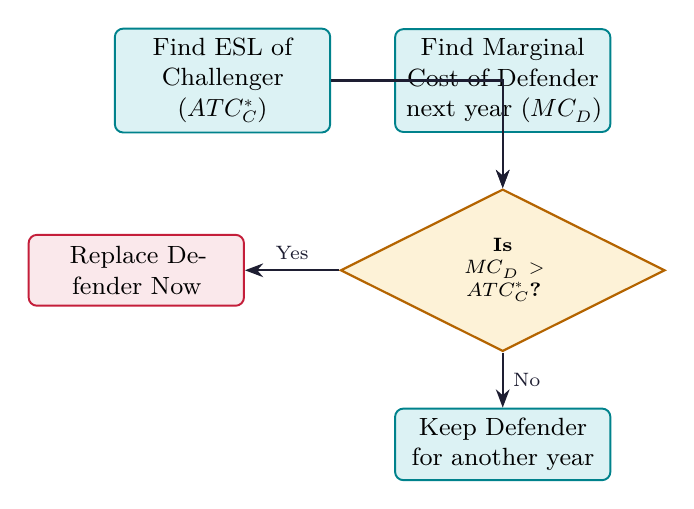
\begin{tikzpicture}[
  node distance=0.4cm and 0.8cm,
  sblock/.style={rectangle, draw=myteal, fill=hdrteal, text width=2.5cm,
    align=center, minimum height=0.9cm, font=\small, rounded corners=3pt, line width=0.7pt},
  rblock/.style={rectangle, draw=myred, fill=hdrred, text width=2.5cm,
    align=center, minimum height=0.9cm, font=\small, rounded corners=3pt, line width=0.7pt},
  decision/.style={diamond, draw=myamber, fill=hdramber, aspect=2, text width=1.8cm,
    align=center, font=\scriptsize\bfseries, line width=0.8pt}
]
  \node[sblock] (n1) {Find ESL of Challenger ($ATC_C^*$)};
  \node[sblock, right=0.8cm of n1] (n2) {Find Marginal Cost of Defender next year ($MC_D$)};
  \node[decision, below=0.7cm of n2] (d1) {Is\\$MC_D > ATC_C^*$?};
  \node[rblock, left=1.2cm of d1] (rep) {Replace Defender Now};
  \node[sblock, below=0.7cm of d1] (keep) {Keep Defender for another year};
  
  \draw[arrow] (n1) -| (d1.north);
  \draw[arrow] (n2) -- (d1.north);
  \draw[arrow] (d1) -- node[above, font=\scriptsize] {Yes} (rep);
  \draw[arrow] (d1) -- node[right, font=\scriptsize] {No} (keep);
\end{tikzpicture}
\end{tcolorbox}

\textbf{Marginal Cost of Defender next year:}
\begin{equation}
  MC_D(t+1) = (MV_t - MV_{t+1}) + (MV_t \times i) + O\&M_{t+1}
\end{equation}
Where $MV_t$ is current market value, $MV_{t+1}$ is market value next year, and $O\&M_{t+1}$ is operating cost next year.

% ===============================================================================
\section{Basic Accounting for Engineers}
% ===============================================================================

Engineers must understand financial statements and cost allocation to make business decisions.

\subsection{Financial Statements}
1.  \textbf{Balance Sheet:} Represents a snapshot of the firm's financial position at a specific point in time. It satisfies the fundamental accounting equation:
    \begin{equation}
      \text{Assets} = \text{Liabilities} + \text{Owner's Equity}
    \end{equation}
2.  \textbf{Income Statement:} Summarizes revenues and expenses over a period of time (e.g., quarter or year) to calculate net income:
    \begin{equation}
      \text{Net Income} = \text{Revenues} - \text{Expenses}
    \end{equation}

\subsection{Financial Ratios}
\begin{itemize}[leftmargin=*, itemsep=6pt]
  \item \textbf{Liquidity (Current Ratio):} $\text{Current Ratio} = \displaystyle\frac{\text{Current Assets}}{\text{Current Liabilities}}$
  \item \textbf{Profitability (Return on Equity):} $ROE = \displaystyle\frac{\text{Net Income}}{\text{Owner's Equity}}$
  \item \textbf{Leverage (Debt-to-Equity):} $\text{Debt-to-Equity} = \displaystyle\frac{\text{Total Liabilities}}{\text{Owner's Equity}}$
\end{itemize}

\subsection{Cost Accounting and Allocation}
\begin{itemize}[leftmargin=*, itemsep=4pt]
  \item \textbf{Direct Costs:} Costs directly traceable to a product or service (e.g., direct materials, assembly labor).
  \item \textbf{Indirect Costs (Overhead):} Costs that cannot be easily traced to a specific product (e.g., building rent, supervisor salaries, factory electricity).
  \item \textbf{Indirect Cost Allocation:} Distributing overhead costs to products using allocation bases like direct labor hours, machine hours, or direct material costs.
\end{itemize}

% ===============================================================================
\section{Worked Examples}
% ===============================================================================

\begin{tcolorbox}[examplebox, title={Example 1: Double Declining Balance (DDB)}]
\textbf{Problem:} A test instrument costs $\$80,000$, has a useful life of $5$ years, and a salvage value of $\$10,000$. Calculate the depreciation amount and book value for Year 1 and Year 2 using the DDB method.\\[4pt]
\textbf{Solution:}
Identify parameters: Cost $C = \$80,000$, Life $n = 5$, Salvage value $S = \$10,000$.
Calculate DDB rate $\alpha$:
\begin{equation*}
  \alpha = \frac{2}{n} = \frac{2}{5} = 0.40 \quad (40\% \text{ per year})
\end{equation*}
\begin{itemize}[leftmargin=*, itemsep=8pt]
  \item \textbf{Year 1:}
    \begin{align*}
      \text{Depreciation: } d_1 &= \alpha \times BV_0 = 0.40 \times 80,000 = \$32,000 \\
      \text{Book Value: } BV_1 &= C - d_1 = 80,000 - 32,000 = \$48,000
    \end{align*}
  \item \textbf{Year 2:}
    \begin{align*}
      \text{Depreciation: } d_2 &= \alpha \times BV_1 = 0.40 \times 48,000 = \$19,200 \\
      \text{Book Value: } BV_2 &= BV_1 - d_2 = 48,000 - 19,200 = \$28,800
    \end{align*}
\end{itemize}
Since $BV_2 = \$28,800 > S = \$10,000$, we do not need to adjust for the salvage value floor yet.\\[4pt]
\textbf{Answer:} Year 1: Depreciation $= \mathbf{\$32,000}$, Book Value $= \mathbf{\$48,000}$. Year 2: Depreciation $= \mathbf{\$19,200}$, Book Value $= \mathbf{\$28,800}$.
\end{tcolorbox}

\begin{tcolorbox}[examplebox, title={Example 2: Replacement Analysis}]
\textbf{Problem:} An existing compressor (defender) has a current market value of $\$5,000$. If kept for another year, its market value will fall to $\$3,500$ and operating costs will be $\$6,500$. A new compressor (challenger) has a minimum annual cost of $\$8,000$. At an interest rate of $10\%$, should the company replace the compressor now?\\[4pt]
\textbf{Solution:}
Calculate the Marginal Cost of the defender ($MC_D$) for next year:
\begin{itemize}[leftmargin=*, itemsep=2pt, topsep=2pt]
  \item Current market value $MV_t = \$5,000$, Market value next year $MV_{t+1} = \$3,500$.
  \item Interest rate $i = 0.10$.
  \item Operating and Maintenance cost $O\&M_{t+1} = \$6,500$.
\end{itemize}
\begin{align*}
  MC_D &= (MV_t - MV_{t+1}) + (MV_t \times i) + O\&M_{t+1} \\
  MC_D &= (5,000 - 3,500) + (5,000 \times 0.10) + 6,500 \\
  MC_D &= 1,500 + 500 + 6,500 = \$8,500
\end{align*}
Compare $MC_D$ next year with the minimum annual cost of the challenger ($ATC_C^* = \$8,000$):
\begin{align*}
  MC_D (\$8,500) &> ATC_C^* (\$8,000) \quad (\text{Keeping defender is more expensive})
\end{align*}
Since the marginal cost of keeping the defender exceeds the annual cost of the challenger, the defender should be replaced.\\[4pt]
\textbf{Answer:} \textbf{Replace now}, as keeping the defender for another year costs $\$8,500$ compared to the challenger's annual cost of $\$8,000$.
\end{tcolorbox}

\begin{tcolorbox}[examplebox, title={Example 3: Indirect Cost Allocation}]
\textbf{Problem:} A workshop incurs factory overhead costs of $\$12,000$. It produces two products: Product A (requires $400$ direct labor hours) and Product B (requires $800$ direct labor hours). Allocate the overhead cost to both products using direct labor hours as the allocation base.\\[4pt]
\textbf{Solution:}
Identify parameters: Total Overhead $= \$12,000$, Total Labor Hours $= 400 + 800 = 1,200$ hours.
Calculate the overhead allocation rate:
\begin{align*}
  \text{Allocation Rate} &= \frac{\text{Total Overhead}}{\text{Total Labor Hours}} = \frac{12,000}{1,200} = \$10 \text{ per labor hour}
\end{align*}
Allocate overhead to each product:
\begin{itemize}[leftmargin=*, itemsep=8pt]
  \item \textbf{Product A:}
    \begin{align*}
      \text{Allocated Overhead} &= 400 \text{ hours} \times \$10/\text{hour} = \$4,000
    \end{align*}
  \item \textbf{Product B:}
    \begin{align*}
      \text{Allocated Overhead} &= 800 \text{ hours} \times \$10/\text{hour} = \$8,000
    \end{align*}
\end{itemize}
Verification: $\$4,000 + \$8,000 = \$12,000$ (total overhead allocated).\\[4pt]
\textbf{Answer:} \textbf{Product A} is allocated \textbf{\$4,000} and \textbf{Product B} is allocated \textbf{\$8,000}.
\end{tcolorbox}

% ===============================================================================
% MANDATORY QUICK REVISION PAGE
% ===============================================================================
\newpage
\begin{center}
  {\large\bfseries\color{myred} Quick Revision --- Module IV}\\[3pt]
  {\small\color{mydark} Depreciation, Replacement \& Accounting $|$ HS-HU601}
\end{center}
\noindent{\color{myred}\rule{\linewidth}{1.2pt}}
\vspace{4pt}

\begin{tcolorbox}[formulabox, title={\textbf{Key Formulas at a Glance}}]
\renewcommand{\arraystretch}{1.3}
\begin{tabularx}{\linewidth}{B{3.8cm} X}
Straight-Line Dep.      & $d_t = \displaystyle\frac{C - S}{n}$ \quad ($BV_t = C - t \times d_t$) \\[6pt]
Declining Balance Dep.  & $d_t = \alpha \times BV_{t-1}$ \quad ($BV_t = C \times (1 - \alpha)^t$) \\[4pt]
DDB Rate                & $\alpha = \displaystyle\frac{2}{n}$ \\[6pt]
Capital Recovery        & $CR(k) = [C - S_k(P/F, i, k)] \times (A/P, i, k)$ \\[4pt]
Defender Marginal Cost  & $MC_D(t+1) = (MV_t - MV_{t+1}) + (MV_t \times i) + O\&M_{t+1}$ \\[4pt]
Accounting Equation     & $\text{Assets} = \text{Liabilities} + \text{Owner's Equity}$ \\[4pt]
Current Ratio           & $\text{Current Ratio} = \displaystyle\frac{\text{Current Assets}}{\text{Current Liabilities}}$
\end{tabularx}
\end{tcolorbox}

\begin{tcolorbox}[defbox, title={\textbf{One-Line Definitions}}]
\begin{itemize}[leftmargin=*, itemsep=2pt, topsep=0pt]
  \item \textbf{Depreciation:} Allocation of an asset's cost over its life to account for wear and tear.
  \item \textbf{Book Value:} Cost of an asset minus accumulated depreciation.
  \item \textbf{Economic Service Life:} The asset life that minimizes total equivalent annual cost.
  \item \textbf{Defender:} An existing asset currently owned and operating.
  \item \textbf{Challenger:} The best replacement candidate available.
  \item \textbf{Balance Sheet:} Statement showing assets, liabilities, and equity at a specific point in time.
  \item \textbf{Income Statement:} Statement showing revenues, expenses, and net profit over a period.
  \item \textbf{Direct Cost:} Expense directly traceable to a product (e.g., labor, raw materials).
  \item \textbf{Indirect Cost:} Expense that cannot be easily traced to a product (e.g., rent, utilities).
\end{itemize}
\end{tcolorbox}

\begin{tcolorbox}[exambox, title={\textbf{Frequently Asked / Viva Questions}}]
\begin{enumerate}[topsep=0pt, label=\textbf{Q\arabic*.}, itemsep=5pt]
  \item \Q{What is the difference between physical deterioration and obsolescence?}
    Physical deterioration is wear and tear due to usage or environmental factors. Obsolescence is the loss of value due to technological progress (newer, better alternatives).
  \item \Q{Explain the Straight-Line depreciation method.}
    It allocates an equal amount of depreciation to each year of the asset's useful life: $d_t = (C-S)/n$.
  \item \Q{What is the salvage value floor rule in Declining Balance methods?}
    An asset cannot be depreciated below its salvage value. Once the book value ($BV_t$) drops to the salvage value ($S$), depreciation must stop.
  \item \Q{Define the Economic Service Life (ESL) of an asset.}
    The period of ownership that minimizes the sum of equivalent annual capital recovery costs and annual operating and maintenance costs.
  \item \Q{What costs are included in the Capital Recovery cost ($CR$) of an asset?}
    The annualized cost of depreciation (loss in asset value) and the interest cost on the capital invested in the asset.
  \item \Q{How is the defender's marginal cost for next year calculated?}
    By adding the projected loss in market value, the interest on its current market value, and the operating and maintenance costs for next year.
  \item \Q{State the decision rule in Defender vs. Challenger replacement analysis.}
    If the marginal cost of keeping the defender for one more year is greater than the minimum annual cost of the challenger, replace the defender immediately.
  \item \Q{State the fundamental accounting equation.}
    $\text{Assets} = \text{Liabilities} + \text{Owner's Equity}$. It forms the basis of the Balance Sheet.
  \item \Q{What is the difference between direct and indirect costs in manufacturing?}
    Direct costs can be traced directly to a product (e.g., material). Indirect costs cannot be traced directly and must be allocated (e.g., factory rent).
  \item \Q{What is the Current Ratio, and what does it measure?}
    Current Assets divided by Current Liabilities. It measures a firm's liquidity (ability to pay off short-term debts).

  \item \Q{Explain the concept of overhead cost allocation.}
    The process of distributing indirect costs (like supervisor salaries or utilities) to different products using an allocation base like direct labor hours.
  \item \Q{What is the Double Declining Balance (DDB) depreciation rate?}
    It is twice the straight-line rate: $\alpha = 2/n$. It represents accelerated depreciation in the early years of asset ownership.
\end{enumerate}
\end{tcolorbox}

\begin{tcolorbox}[tikzbox, title={Comparison of Depreciation Methods}]
\renewcommand{\arraystretch}{1.45}
\par\noindent
\begin{tabularx}{\linewidth}{|B{2.3cm}|Y|Y|Y|}
\hline
\textbf{Method} & \textbf{Depreciation Pattern} & \textbf{Calculation Base} & \textbf{Primary Use} \\
\hline
\textbf{Straight-Line} & Constant annual depreciation & $(C-S)$ is constant & Standard accounting; simple financial reporting. \\
\hline
\textbf{Declining Balance} & Accelerated; higher in early years & Remaining book value ($BV_{t-1}$) & Assets that lose value quickly (vehicles, computers). \\
\hline
\textbf{Double Declining} & Maximum acceleration rate ($2/n$) & Remaining book value ($BV_{t-1}$) & Tax reporting (maximizes early tax shields). \\
\hline
\textbf{Sinking Fund} & Increases over time & $(C-S)$ with interest & Special asset funds; rarely used in modern tax accounting. \\
\hline
\end{tabularx}
\end{tcolorbox}

\end{document}
